
\hl{
由于 CNN 缺少旋转不变性,现有的方法就只能使用大量的数据来进行训练,这样才能代表所有可能出现的情况(例如旋转,裁剪等等).
我们推测,对于生物医学图像来说,如果我们先将感兴趣的结构检测处理,然后变换到一个典型方向,则可以更加高效地进行分割.
}
所谓的典型方向(\CMR{})是针对不同的标准切面进行定义的(图 \ref{fig:canonical-orientation}).
我们提出的心脏 \SSFP{} 图像分割网络是端到端训练的,而且允许定位、对齐和分割任务互相影响促进.
我们的模型由三个阶段组成.
第一,将全尺寸的原始图像 $\image$ 输入到一个 \UNet{} 模块 (\S \ref{sec:unet}) 进行粗分割. 
第二,利用 \UNet{} 中间(下采样)的特征来预测一个刚体仿射变换矩阵 $\tmat$,将图像变换到一个典型方向 $\timage = \trans(\image, \tmat)$ (\S\ref{sec:stn}).
第三,用一个堆叠的沙漏形模块(\S\ref{sec:hourglass})对变换后的图像 $\timage$ 进行分割.
以下小节将对每个模块进行详细的讨论.
为了方便,我们在字母上加个小帽表示真实值(如 $\hat{x}$),在字母上加一撇表示预测值(如 $x^\prime$).

\subsection{粗分割 (\UNet{}) 模块}\label{sec:unet}

\renewcommand{\captiontitle}{\UNet{} 模块}
\begin{figure}
\centering
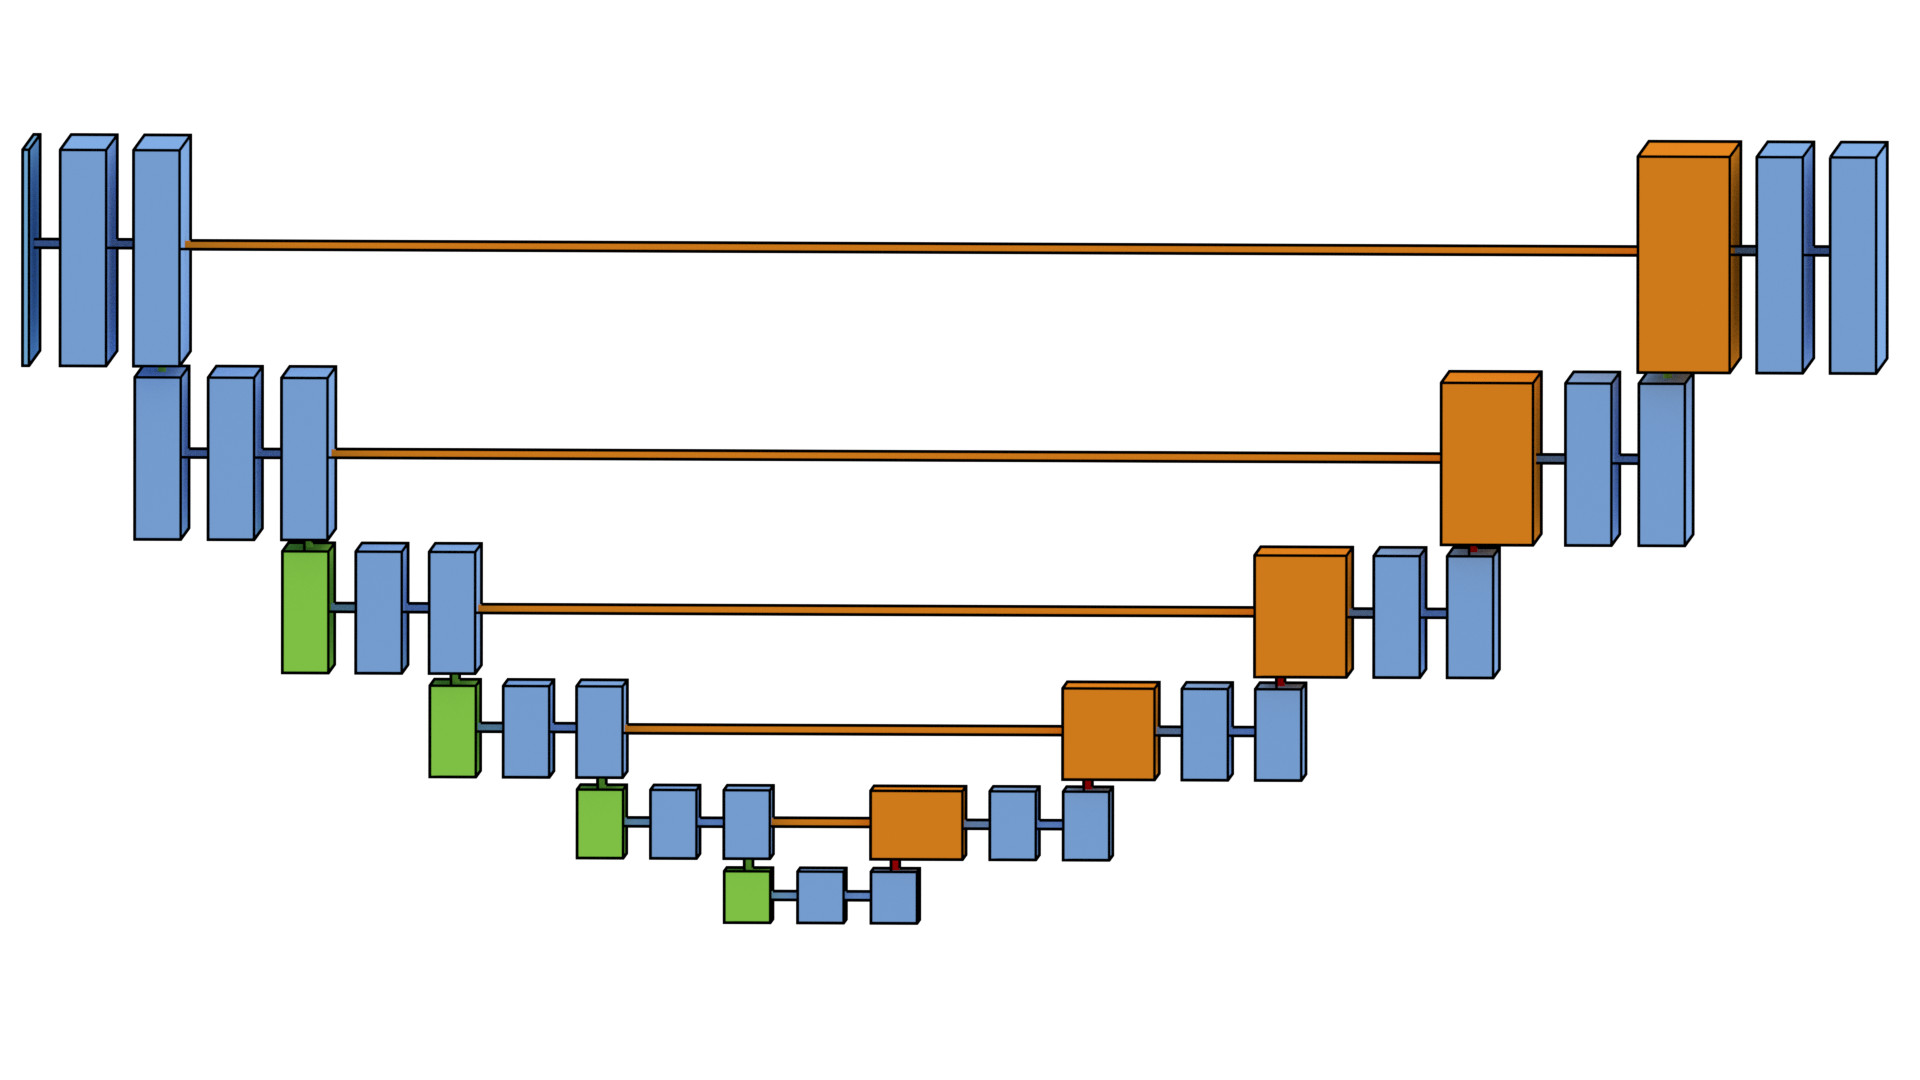
\includegraphics[clip, trim=0 0 0 0,width=0.5\textwidth]{./data/unet-module.png}
\caption[\captiontitle]{\captiontitle{}.  输入图像尺寸为 $\N \times \N \times N$,其中 $N$ 通道数(所有网络的通道数均为 $1$).
蓝色、绿色和橙色方框对应着多通道的特征图.绿色对应的是下采样的特征图,橙色对应的是将结果与特征图的拼接.}
\label{fig:unet-module}
\end{figure}



本文提出的网络使用了一个在生物医学图像分割任务\citep{Long2015,Ronneberger2015,Xie2015}中表现优异的深度卷积神经网络 \UNet{} 模块(图 \ref{fig:unet-module}).
\UNet{} 模块由左侧的下采样和右侧的上采样组成.
下采样部分由一个典型的 CNN 网络 \citep{Krizhevsky2012,Simonyan2015} 组成,两个 $3 \times 3$ 的卷积层,一个 \ReLU{} 激活层,一个 $2 \times 2$ 的最大化池化层,这些层不断重复堆叠,应用到输入图像和特征图.
下采样部分,经过不断的 $2 \times 2$ 上采样,\ReLU{} 激活和 $3 \times 3$ 卷积,下采样的图像恢复到原来的尺寸.
为了提供更加准确的分割边界,我们使用了跳跃连接,使得相同层级的下采样和下采样的输出串联到一起.
批标准化 \mbox{\citep{Ioffe2015}} 已经被证明可以有效地避免梯度消失现象,所以我们在每一个卷积层与激活层之间均加入了批标准化操作.
\UNet{} 模块的损失函数 $L_{S_U}$ 为交叉熵损失函数,也就是输出 $P$ 与真实值 $\hat{S}$ 的交叉熵,

\begin{equation}\label{eqn:unet-loss}
L_{S_U} = -\frac{1}{HW} \sum_{\forall h,w} \CCE(P_{h,w}, \hat{S}_{h,w}),
\end{equation}

\noindent 其中

\begin{equation}\label{eqn:cross-entropy}
\CCE(x, \hat{x}) = - \hat{x} \log(x) + (1 - \hat{x}) \log(1 - x).
\end{equation}

\hl{
$H$ 和 $W$ 分别为输入图像的高度和宽度,$h$ 和 $w$ 为对应的索引.
}

\subsection{\hl{变换} 模块}\label{sec:stn}

\renewcommand{\captiontitle}{空间变换网络模块}
\begin{figure}
\begin{center}

\begin{tikzpicture}
\node [anchor=south west] (image) at (0,0) {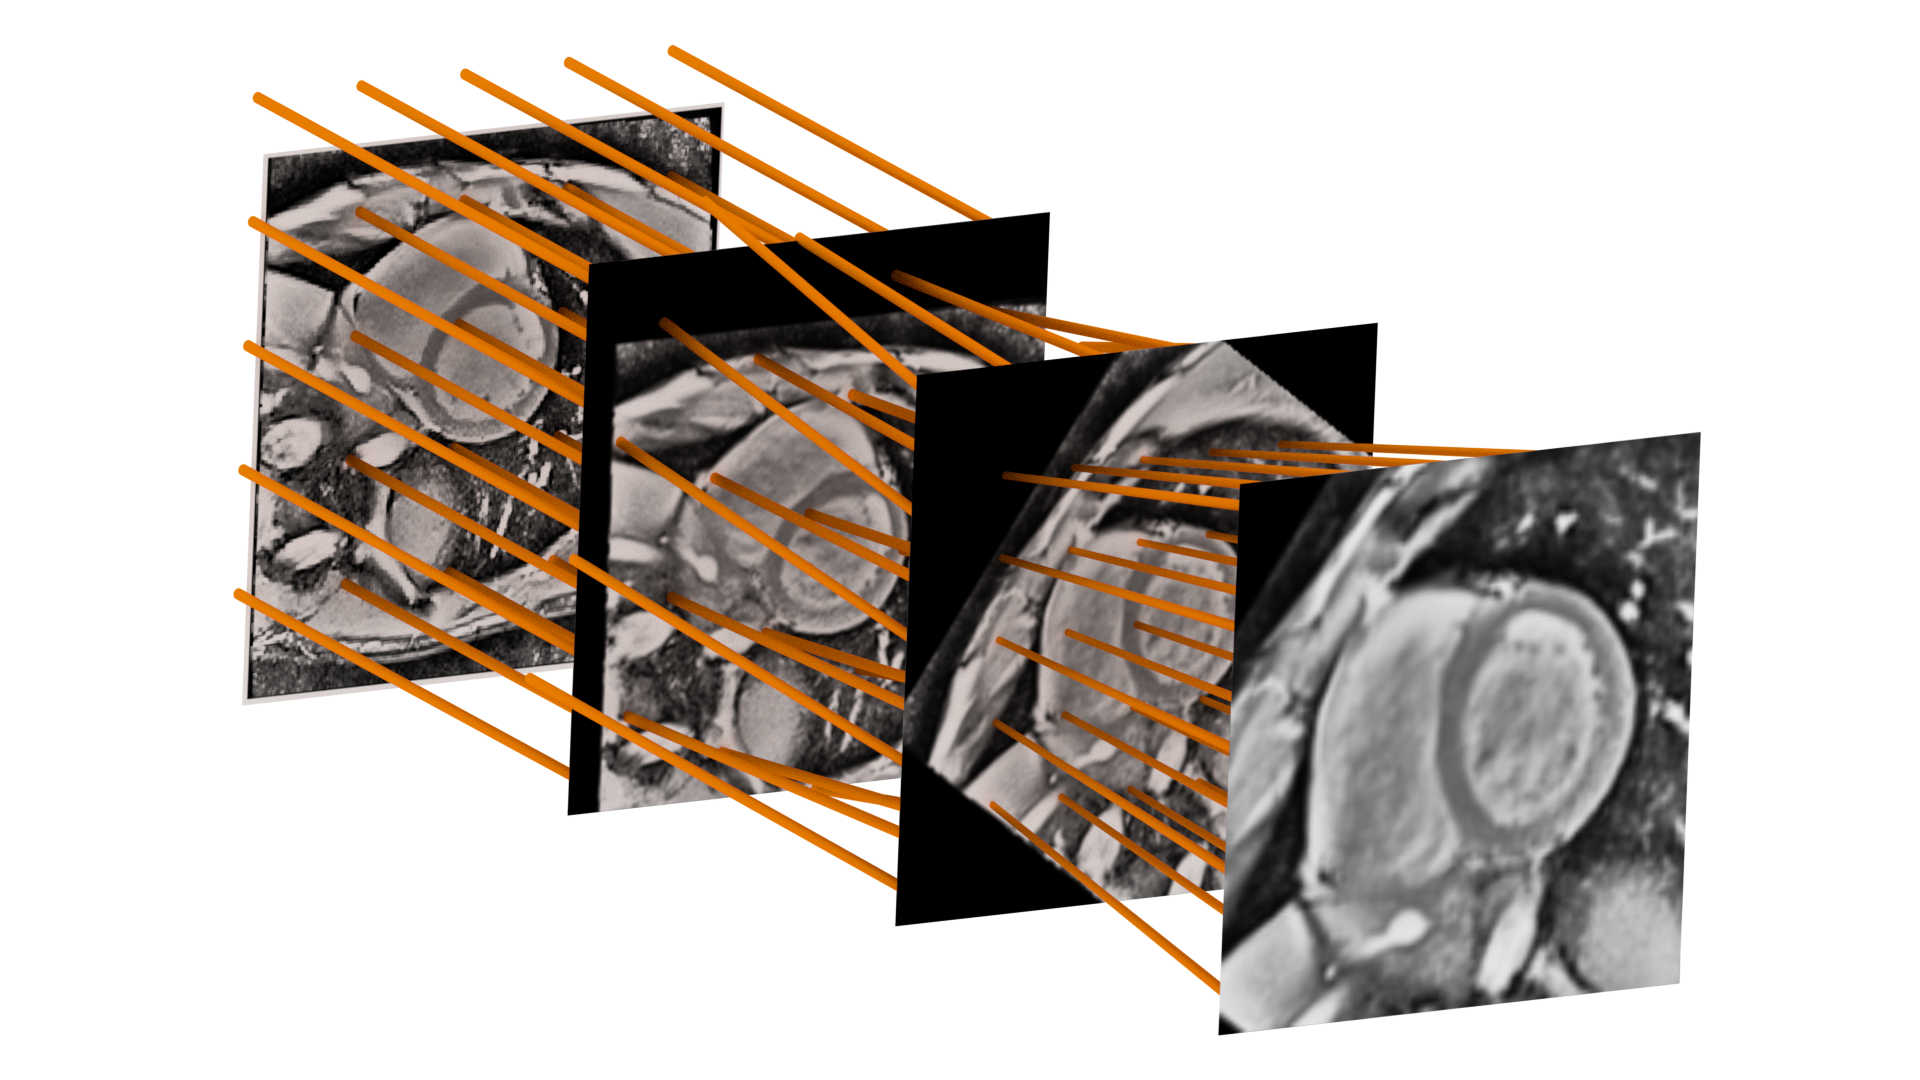
\includegraphics[width=0.5\textwidth]{./data/sampler.png}};
\draw [decorate,decoration={brace,amplitude=10pt},xshift=0pt,yshift=0pt](2.8,1.317) -- (1.25,1.85) node [black,midway,xshift=-0.3cm,yshift=-0.7cm] {\footnotesize $\image_2 = \trans(\image, T)$};
\draw [decorate,decoration={brace,amplitude=10pt},xshift=0pt,yshift=0pt](4.35,0.783) -- (2.8,1.317) node [black,midway,xshift=-0.3cm,yshift=-0.7cm] {\footnotesize $\image_3 = \trans(\image_2, R)$};
\draw [decorate,decoration={brace,amplitude=10pt},xshift=0pt,yshift=0pt](5.9,0.25) -- (4.35,0.783) node [black,midway,xshift=-0.3cm,yshift=-0.7cm] {\footnotesize $\trans(\image_3, S)$};
\end{tikzpicture}

\caption[\captiontitle]{\captiontitle{}.请注意,在实际的实现中,所有的变换都是相对于输入图像 $\image$ (即 $\trans(\image, T)$,$\trans(\image, RT)$和$\trans(\image, SRT)$)的变换;我们在此处只是为了清晰地说明这是连续处理的步骤.}
\label{fig:stn-module}
\end{center}
\end{figure}



空间变换网络(\STN{}) 最初是作为分类任务的通用层提出的,目的是提升空间不变性\citep{Jaderberg2015}.
\STN{} 模块本身由三个子模块组成:一个定位模块(\LocNet{})模块,用于预测一个刚体仿射变换矩阵 $\tmat$;一个网格生成器,用于实现变换 $\trans$;一个采样器,用于实现插值.

在文献 \citep{Jaderberg2015} 中,\STN{} 网络可以学习到适合分类任务的最佳变换参数;而且也不需要给出真实值,预测的变换矩阵用于将中间层的\emph{特征图}进行变换.
但是,在本文的应用中,我们感兴趣的是学习如何将\emph{输入图像}变换到一个标准的临床方向,从而指引语义分割任务.

%%%%%%%%%%%%%%%%%%%%%%%%%%%%%%%%%%%%%%%%%%
% 	Locnet
%%%%%%%%%%%%%%%%%%%%%%%%%%%%%%%%%%%%%%%%%%
\subsubsection{定位网络(\LocNet{})}

给出一个心脏分割图像,一个人类专家可以从直觉上给出平移、旋转和缩放信息.
基于这一假设,我们从 \UNet{} 的最后一个最大化池化层的输出引出一个小小的定位网络(\LocNet{})分支,从而预测变换参数(图 \ref{fig:stn-module}).
我们将变换限定为平移、旋转和缩放,则仿射变换矩阵可以分解为三个矩阵:

$$
\tmat = SRT,
$$

\noindent 其中 $T$ 为平移变换矩阵:

$$
T =
\begin{bmatrix}
1 & 0 & t_x \\
0 & 1 & t_y \\
0 & 0 & 1 \\
\end{bmatrix};
$$

\noindent $R$ 为旋转变换矩阵(逆时针):

$$
R =
\begin{bmatrix}
\cos(\theta) & - \sin(\theta) & 0 \\
\sin(\theta) & \cos(\theta) & 0 \\
0 & 0 & 1 \\
\end{bmatrix};
$$

\noindent 以及 $S$ 为缩放变换矩阵:

$$
S =
\begin{bmatrix}
s & 0 & 0 \\
0 & s & 0 \\
0 & 0 & 1 \\
\end{bmatrix}.
$$

\noindent 图像定义在一个归一化的坐标空间 $\{x, y\} \in [-1, +1]$,这样它的旋转是相对于图像中心点来说的.

定位网络 \LocNet{} 只需要学习和预测相关的参数 $\tparams = \begin{bmatrix}t_x & t_y & \theta & s \end{bmatrix}^\top$.
我们在训练中提供真实值 $\hat{\tparams} = \begin{bmatrix} \hat{t_x} & \hat{t_y} & \hat{\theta} & \hat{s} \end{bmatrix}$,并不断地最小化两个损失,即 \emph{矩阵损失(matrix losses)}和\emph{图像损失(image losses)}.

矩阵损失为真实值与预测值 $L_{t_x}$, $L_{t_y}$, $L_\theta$, $L_s$ 之间的回归损失.
对于缩放和平移来说,我们使用了均方根误差(\MSE{})作为损失函数:

\begin{align}
L_{t_x} & = \frac{1}{2} (t_x - \hat{t_x})^2, \label{eqn:attn-mat-loss-tx} \\
L_{t_y} & = \frac{1}{2} (t_y - \hat{t_y})^2, \mathrm{~and} \label{eqn:attn-mat-loss-ty} \\
L_s     & = \frac{1}{2} (s - \hat{s})^2. \label{eqn:attn-mat-loss-s}
\end{align}

\renewcommand{\captiontitle}{均方根误差(\MSE{}) vs 包裹的均方根误差(\MSWE{})}
\begin{figure*}
\begin{center}
\begin{subfigure}{0.48\textwidth}
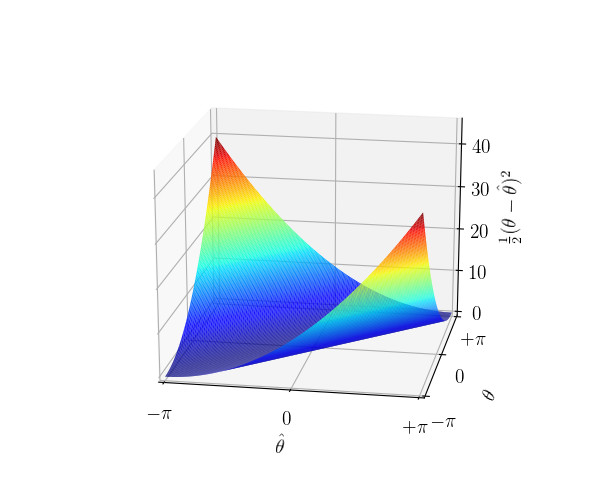
\includegraphics[clip, trim=90 30 50 70,width=1.0\textwidth]{./data/phase-loss.png}
\caption{均方根误差(\MSE{})}
\end{subfigure}
\begin{subfigure}{0.48\textwidth}
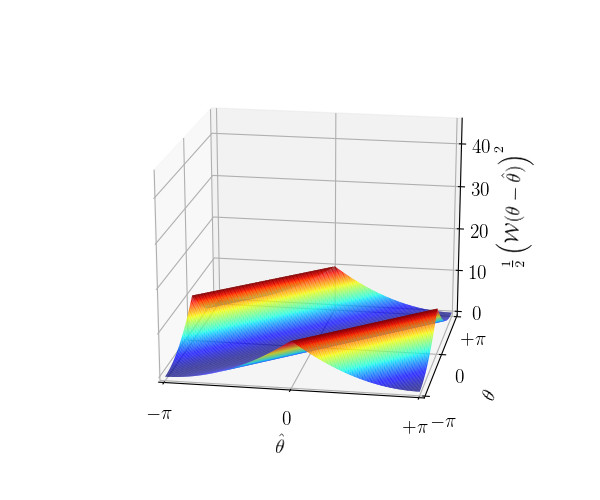
\includegraphics[clip, trim=90 30 50 70,width=1.0\textwidth]{./data/wrapped-phase-loss.png}
\caption{包裹的均方根误差(\MSWE{})}
\end{subfigure}
\caption[\captiontitle]{\captiontitle{}.}
\label{fig:wrapped-phase-loss}
\end{center}
\end{figure*}



由于周期性,简单的 \MSE{} 并不适合作为参数 $\theta$ 的损失函数.举例来说,当预测值为 $\theta = -\pi$,真实值为 $\hat{\theta} = \pi$ 的时候,\MSE{} 的损失值也最大.
因此,我们提出一个包裹的 \MSE{} 损失函数(\MSWE{}),如图 \ref{fig:wrapped-phase-loss} 所示,我们将 $\theta - \hat{\theta}$ 包裹起来,使其取值范围为 $[-\pi, \pi)$,然后再用标准的 \MSE{} 计算,

\begin{equation}
L_\theta = \frac{1}{2} \left(\wrap(\theta - \hat{\theta})\right)^2, \label{eqn:attn-mat-loss-r}
\end{equation}

\noindent 其中这个包裹的操作 $\wrap$ 定义为

$$
\wrap(\cdot) = \mod(\cdot + \pi, 2\pi) - \pi.
$$

仅仅基于这些损失进行变换模块的训练很容易导致过拟合.
为此,我们基于 \MSE{} 额外添加了变换后的图像的真实值$\hat{\tparams}$与预测值$\tparams$之间的正则化约束项:

\begin{align}
L_{\image_t}      & = \frac{1}{2} (\trans(\image, T  ) - \trans(\image, \hat{T}  ))^2,                     \label{eqn:attn-image-loss-t} \\
L_{\image_\theta} & = \frac{1}{2} (\trans(\image, RT ) - \trans(\image, \hat{R}\hat{T} ))^2, \mathrm{~and} \label{eqn:attn-image-loss-r} \\
L_{\image_s}      & = \frac{1}{2} (\trans(\image, SRT) - \trans(\image, \hat{S}\hat{R}\hat{T}))^2.         \label{eqn:attn-image-loss-s}
\end{align}

%%%%%%%%%%%%%%%%%%%%%%%%%%%%%%%%%%%%%%%%%%
% 	Sampler
%%%%%%%%%%%%%%%%%%%%%%%%%%%%%%%%%%%%%%%%%%
\subsubsection{网格生成和采样}

一般来说,一个 \ND{2} 网格生成器均匀采样 $G \in \Real^{2 \times H' \times W'}$,然后根据 \LocNet{} 预测的参数对他们进行变换.
在我们的应用中,我们生成三个这样的网格,每个的维度等于输入($H' = W' = \N$),并均匀延伸到图像大小($x \in [-1,1]$, $y \in [-1, 1]$).
随后,我们用 \LocNet{} 预测的参数$T$,$RT$和$SRT$将这些网格进行变换,从而确定原始图像中的哪些点需要采样.

采样器的输入参数为输入图像 $\image \in \Real^{H \times W \times C}$ 和变换网格 $G^\prime$,输出为一个重采样的图像 $\timage \in \Real^{H' \times W' \times C}$.
\footnote{\hl{为了完整性,我们引入了通道参数 $C$;然而,应该强调的是,我们的应用中输入为灰度图 $\image$,也就是 $C = 1$ 的情况.}}
对于每一个通道 $c \in [1 \twodots C ]$,$(h',w')$ 处的输出 $\timage_{h',w',c}$ 为输入值 $\image_{h,w,c}$ 在邻域 $G^\prime_{1,h',w'}, G^\prime_{2,h',w'}$ 的加权和,

\begin{align*}
\timage_{h',w',c} & = \sum^H_{h=1}\sum^W_{w=1}\image_{h, w, c} \\
                  & \cdot \max\left(0, 1-|\alpha_v G^\prime_{1, h', w'} + \beta_v - h| \right) \\
                  & \cdot \max\left(0, 1-|\alpha_u G^\prime_{2, h', w'} + \beta_u - w| \right),
\end{align*}

\noindent 其中

$$
\begin{aligned}
\alpha_v & = +\frac{H-1}{2},               \\
\beta_v  & = -\frac{H+1}{2},              \\
\alpha_u & = +\frac{W-1}{2}, \mathrm{ and} \\
\beta_u  & = - \frac{W+1}{2}.
\end{aligned}
$$

\noindent 这里的每一步计算都是可微的,这样就保证了模型可以端到端地进行训练.

%%%%%%%%%%%%%%%%%%%%%%%%%%%%%%%%%%%%%%%%%%
% 	Hourglass
%%%%%%%%%%%%%%%%%%%%%%%%%%%%%%%%%%%%%%%%%%
\subsection{细分割模块(堆叠的沙漏形网络)}\label{sec:hourglass}

变换模块的输出是已经变换到一个典型方向的了,接着就是送入一个堆叠的沙漏形网络结构中.
这个沙漏形网络由 $D = [1 \twodots 3]$ 个 \UNet{} 模块前后连接而成.每个 \UNet{} 模块产生一个分割输出 $S_{H,d}$,其中 $d \in [1 \twodots D]$.
第 $d$ 层的输出 $P^{H,d}_{h,w}$ 与真实值 $\hat{S}^\prime$ 的交叉熵可以按照公式 \eqref{eqn:cross-entropy} 进行计算,

\begin{equation}\label{eqn:hourglass-loss}
L_{S_{H,d}} = -\frac{1}{HW} \sum_{\forall h,w} \CCE(P^{H,d}_{h,w}\hat{S}^\prime_{h,w}).
\end{equation}

%%%%%%%%%%%%%%%%%%%%%%%%%%%%%%%%%%%%%%%%%%
% 	Summary
%%%%%%%%%%%%%%%%%%%%%%%%%%%%%%%%%%%%%%%%%%
\subsubsection{小结}

小结一下,我们使用损失函数公式 \ref{eqn:unet-loss} 来训练 \omeganet{} 的粗分割模块;四个矩阵损失函数公式 \ref{eqn:attn-image-loss-t}、\ref{eqn:attn-image-loss-r}和\ref{eqn:attn-image-loss-s}来训练变换模块;以及一到三个损失函数公式 \ref{eqn:hourglass-loss} 来训练最后的细分割模块.
因此,总的损失函数就是:

\begin{equation}
\begin{aligned}
L_\Omega & = \alpha_1 L_{S_U} \\
  & + \alpha_2 (L_{t_x} + L_{t_y} + L_{\theta}+ L_{s}) \\
  & + \alpha_3 (L_{I_t} + L_{I_\theta} + L_{I_s}) \\
  & + \alpha_4 \sum_{d=1}^D L_{S_{H,d}}, \\
\end{aligned}
\end{equation}

\noindent 其中 $\alpha_1 = 100.0$,$\alpha_2 = 100.0$,$\alpha_3 = 0.1$,$\alpha_4 = 1.0$.
网络结构总结如表 \ref{tab:architecture-descriptions} 所示.

\hl{
尽管我们的输入数据经过了较小的刚体仿射变换进行数据增强,我们还要特别指出的是,细分割期间也进行了\emph{隐含的}数据增强,因为我们在粗分割的时候使用了变换网络.
}
